\section{Multivariate random variables}
\label{sec:multivariate}

\noindent\textbf{Primary reading.} Freund, Chapter 3, \S5 ``Multivariate Distributions,'' pp.~82--91; \S6 ``Marginal Distributions,'' pp.~92--95; \S7 ``Conditional Distributions,'' pp.~95--101. In Freund, $g(x)$ and $h(y)$ often denote the two marginals; here we write $p_X,p_Y$ or $f_X,f_Y$ to show which variable is retained. The word \emph{distribution} can mean the entire probability law. A \emph{distribution function} means a CDF; it is not the same object as a PMF or PDF.

\begin{quote}
\textbf{Read with a purpose.} In \S5, study Example~13 (p.~83) for normalization, Example~16 (pp.~86--87) for a full piecewise CDF, and the rectangle-increment task in Exercise~58 (p.~91). In \S6, study Example~21 (p.~93) for marginal densities. In \S7, compare Example~24 (pp.~96--97), where conditioning changes the law, with Example~25 (pp.~97--98), where it does not. This comparison explains independence more clearly than memorizing the product rule alone.
\end{quote}

\subsection{Joint laws, support, and normalization}

A random vector $(X,Y)$ records two numerical measurements from the same experiment. Its \textbf{support} describes the pairs that can occur. Write the support before calculating: the formula alone does not specify the model.

For discrete variables, the joint probability mass function is
\[
 p_{X,Y}(x,y)=P(X=x,Y=y),\qquad
 p_{X,Y}(x,y)\geq0,\qquad \sum_x\sum_y p_{X,Y}(x,y)=1.
\]
The comma inside $P(X=x,Y=y)$ means ``and.'' Sum only over allowed pairs. A probability table is a joint PMF written as a grid.

For an absolutely continuous random vector, the joint probability density satisfies
\[
 f_{X,Y}(x,y)\geq0,\qquad
 \iint_{\mathbb R^2}f_{X,Y}(x,y)\,\dd x\,\dd y=1,
 \qquad
 P((X,Y)\in A)=\iint_A f_{X,Y}(x,y)\,\dd x\,\dd y.
\]
The density is zero off its support. A density is \emph{probability per unit area}; its value need not be at most one. In an absolutely continuous model, $P(X=x,Y=y)=0$, and lines such as $X=Y$ also have probability zero. The latter statement need not hold for a random vector concentrated on a line, even if each individual variable is continuous.

\paragraph{Finding an unknown constant.} If $p(x,y)=c\,w(x,y)$ on a finite support $S$, then
\[
 c=\left[\sum_{(x,y)\in S}w(x,y)\right]^{-1}.
\]
For a continuous density, replace the sum by the integral over $S$. Check nonnegativity as well as total mass. If the proposed formula changes sign, a normalizing constant alone cannot repair it.

\subsubsection*{Worked example: turn a formula into a joint table}
Let $p(x,y)=c(1+x+2y)$ for $x\in\{0,1\}$ and $y\in\{0,1,2\}$, and zero otherwise. The six weights add to $1+3+5+2+4+6=21$, so $c=1/21$:
\[
\begin{array}{c|ccc|c}
 &y=0&y=1&y=2&p_X(x)\\\hline
x=0&1/21&3/21&5/21&9/21\\
x=1&2/21&4/21&6/21&12/21\\\hline
p_Y(y)&3/21&7/21&11/21&1
\end{array}
\]
For example, $P(X>Y)=p(1,0)=2/21$. The event $X+Y\leq1$ contains exactly $(0,0),(0,1),(1,0)$, giving $P(X+Y\leq1)=6/21=2/7$.

\paragraph{Checkpoint.} Find $c$ for $p(x,y)=cxy$ on $x\in\{1,2\}$, $y\in\{1,2\}$, and then find $P(X=Y)$. \emph{Answer:} $c=1/9$ and $P(X=Y)=(1+4)/9=5/9$.

\subsection{Joint CDFs and recovering probabilities}

For either type of random vector,
\[
 F_{X,Y}(x,y)=P(X\leq x,Y\leq y).
\]
Thus a CDF gives the probability in the lower-left rectangle ending at $(x,y)$. A CDF is defined for every real $(x,y)$, takes values in $[0,1]$, is nondecreasing in either coordinate with the other fixed, and has nonnegative probability increments over rectangles. The last condition matters: being increasing in each coordinate alone is not enough to guarantee a valid joint CDF.

\[
\begin{aligned}
\text{Discrete:}\quad
F_{X,Y}(x,y)&=\sum_{s\leq x}\sum_{t\leq y}p_{X,Y}(s,t),\\
\text{Continuous:}\quad
F_{X,Y}(x,y)&=\int_{-\infty}^{x}\int_{-\infty}^{y}
f_{X,Y}(s,t)\,\dd t\,\dd s.
\end{aligned}
\]
For an absolutely continuous law, recover the density by
\[
 f_{X,Y}(x,y)=\frac{\partial^2 F_{X,Y}(x,y)}{\partial x\,\partial y}
 \quad\text{almost everywhere}.
\]
Differentiate only the appropriate branch and preserve its support. A density formula inside the support is not the full CDF.

\paragraph{Rectangle probabilities from a CDF.} Inclusion--exclusion gives the identity
\[
\boxed{\begin{aligned}
P(a<X\leq b,\ c<Y\leq d)
={}&F(b,d)-F(a,d)-F(b,c)+F(a,c).
\end{aligned}}
\]
This identity holds for arbitrary laws. For a continuous joint density, changing strict to non-strict inequalities does not change the answer. For discrete variables, endpoints matter: if $X,Y$ are integer valued,
\[
\begin{aligned}
P(a\leq X\leq b,c\leq Y\leq d)
={}&F(b,d)-F(a-1,d)-F(b,c-1)+F(a-1,c-1)
\end{aligned}
\]
for integer endpoints. At an isolated mass point, the PMF is the CDF's two-dimensional jump. On an integer grid,
\[
 p(x,y)=F(x,y)-F(x-1,y)-F(x,y-1)+F(x-1,y-1).
\]
For a non-integer discrete support, use left limits at the point, rather than blindly subtracting one.

\subsubsection*{Worked example: a CDF with every boundary covered}
Let
\[
 f(x,y)=\frac32(x^2+y^2),\quad 0<x<1,\ 0<y<1,
 \qquad f(x,y)=0\text{ otherwise}.
\]
The integral of $x^2+y^2$ over the unit square is $2/3$, so this is normalized. In the interior,
\[
 F(x,y)=\int_0^x\int_0^y\frac32(s^2+t^2)\,\dd t\,\dd s
 =\frac12(x^3y+xy^3).
\]
The integration must stop at the edge of the support. The complete answer is
\[
F(x,y)=
\begin{cases}
0,&x\leq0\text{ or }y\leq0,\\
\tfrac12(x^3y+xy^3),&0<x<1,\ 0<y<1,\\
\tfrac12(y+y^3),&x\geq1,\ 0<y<1,\\
\tfrac12(x+x^3),&0<x<1,\ y\geq1,\\
1,&x\geq1,\ y\geq1.
\end{cases}
\]
All boundaries agree with their adjacent branches. A compact check is to set $u=\min(1,\max(0,x))$ and $v=\min(1,\max(0,y))$; then $F(x,y)=(u^3v+uv^3)/2$. In the interior, differentiating twice returns $\tfrac32(x^2+y^2)$.

\paragraph{Checkpoint.} For the CDF above, find $P(X\leq1/2,Y>1/2)$. \emph{Answer:} $F(1/2,1)-F(1/2,1/2)=5/16-1/16=1/4$.

\subsection{Marginals: integrate or sum out the other variable}

The marginal law of $X$ describes $X$ with $Y$ unobserved. It is not obtained by inserting a convenient value of $y$ into the joint law:
\[
\begin{array}{ll}
\text{Discrete:}&p_X(x)=\displaystyle\sum_y p_{X,Y}(x,y),\quad
p_Y(y)=\displaystyle\sum_x p_{X,Y}(x,y),\\[5pt]
\text{Continuous:}&f_X(x)=\displaystyle\int_{-\infty}^{\infty}f_{X,Y}(x,y)\,\dd y,\quad
f_Y(y)=\displaystyle\int_{-\infty}^{\infty}f_{X,Y}(x,y)\,\dd x.
\end{array}
\]
\textbf{Keep the variable named in the subscript; eliminate the other one.} The surviving variable is a parameter during the integration. State the marginal's support and put it equal to zero elsewhere.

From the joint CDF,
\[
 F_X(x)=\lim_{y\to\infty}F_{X,Y}(x,y),\qquad
 F_Y(y)=\lim_{x\to\infty}F_{X,Y}(x,y).
\]
Once a marginal is known, compute its univariate probabilities by summing, integrating, or subtracting CDF values.

\subsubsection*{Worked example: support-dependent marginal bounds}
Suppose
\[
 f(x,y)=8xy\quad\text{on }0<x<y<1,
 \qquad f(x,y)=0\text{ elsewhere}.
\]
For fixed $x$, the allowed values of $y$ run from $x$ to $1$. For fixed $y$, the allowed values of $x$ run from $0$ to $y$. Consequently,
\[
\begin{aligned}
 f_X(x)&=\int_x^1 8xy\,\dd y=4x(1-x^2),&&0<x<1,\\
 f_Y(y)&=\int_0^y 8xy\,\dd x=4y^3,&&0<y<1.
\end{aligned}
\]
Both densities integrate to one. The calculation also verifies that the original joint density is normalized. Using $\int_0^1$ for the first marginal would incorrectly include points with $y<x$ where the joint formula does not apply.

\paragraph{Checkpoint.} For $f(x,y)=2$ on $0<x<y<1$, find both marginals. \emph{Answer:} $f_X(x)=2(1-x)$ and $f_Y(y)=2y$ on $(0,1)$, zero otherwise.

\subsection{Conditional laws and reconstructing a joint law}

A conditional law describes the remaining uncertainty after one variable is fixed. Divide by the marginal of the \emph{given} variable:
\[
\boxed{p_{X\mid Y}(x\mid y)=\frac{p_{X,Y}(x,y)}{p_Y(y)}}\quad(p_Y(y)>0),
\qquad
\boxed{f_{X\mid Y}(x\mid y)=\frac{f_{X,Y}(x,y)}{f_Y(y)}}\quad(f_Y(y)>0).
\]
For fixed $y$, sum or integrate over $x$ and check that the answer is one. The conditional support is the slice of the original support at that $y$.

In a continuous model, $P(Y=y)=0$. The conditional density formula defines the usual density-based conditional law; it is \emph{not} literal division by the probability $P(Y=y)$. If the question gives an interval event such as $Y\in B$ instead, use
\[
 P(X\in A\mid Y\in B)
 =\frac{\displaystyle\int_B\int_A f_{X,Y}(x,y)\,\dd x\,\dd y}
 {\displaystyle\int_B f_Y(y)\,\dd y},
 \qquad P(Y\in B)>0.
\]
Restrict both integrals to the support. Conditioning on $Y\leq1/2$ is different from conditioning on $Y=1/2$.

\paragraph{Conditional CDF.} Once the conditional PMF or PDF is available,
\[
 F_{X\mid Y}(a\mid y)=\sum_{x\leq a}p_{X\mid Y}(x\mid y)
 \quad\text{or}\quad
 F_{X\mid Y}(a\mid y)=\int_{-\infty}^{a}f_{X\mid Y}(x\mid y)\,\dd x.
\]
For a sufficiently smooth absolutely continuous law with $f_Y(y)>0$,
\[
 F_{X\mid Y}(a\mid y)
 =\frac{\partial F_{X,Y}(a,y)/\partial y}{f_Y(y)}.
\]
Integrating the conditional PDF is usually the safest route on an exam.

\subsubsection*{Worked example: a conditional slice}
For the square density $\tfrac32(x^2+y^2)$ used above,
\[
 f_Y(y)=\frac12+\frac32y^2,
 \qquad
 f_{X\mid Y}(x\mid y)=\frac{3(x^2+y^2)}{1+3y^2},\quad0<x<1,
\]
for $0<y<1$. Thus
\[
 P\left(X\leq\frac12\,\middle|\,Y=\frac12\right)
 =\int_0^{1/2}\frac{12x^2+3}{7}\,\dd x=\frac27.
\]
For the triangular density $8xy$, instead,
\[
 f_{Y\mid X}(y\mid x)=\frac{8xy}{4x(1-x^2)}
 =\frac{2y}{1-x^2},\qquad x<y<1,\quad0<x<1.
\]
Its support depends on $x$; ignoring that dependence would change the conditional law.

\paragraph{Which directions of conversion are possible?}
\begin{itemize}[leftmargin=*]
\item Joint law $\longrightarrow$ either marginal or either conditional: sum/integrate and divide, where the relevant denominator is positive.
\item Marginal $+$ matching conditional $\longrightarrow$ joint law:
\[
 f_{X,Y}(x,y)=f_{X\mid Y}(x\mid y)f_Y(y)
 =f_{Y\mid X}(y\mid x)f_X(x),
\]
with the analogous PMF identities. Preserve both the marginal support and conditional slice support.
\item Two marginals alone do \emph{not} determine a joint law. They describe individual behavior but leave dependence unspecified. If independence is additionally established, multiply the marginals.
\item One conditional law alone generally does not determine the joint law; the distribution of the conditioning variable is still missing.
\end{itemize}
For example, a Bernoulli$(1/2)$ pair can be independent, equal almost surely ($Y=X$), or opposite almost surely ($Y=1-X$). Every case has the same two marginals, but the joint probabilities differ.

\paragraph{Checkpoint.} Suppose $f_Y(y)=2y$ on $(0,1)$ and, given $Y=y$, $X$ is uniform on $(0,y)$. Find the joint density and $f_X$. \emph{Answer:} $f_{X,Y}(x,y)=2$ on $0<x<y<1$, and $f_X(x)=2(1-x)$ on $(0,1)$.

\subsection{Independence: what must be proved}

Independence means that knowing either variable gives no information about the other:
\[
 P(X\in A,Y\in B)=P(X\in A)P(Y\in B)
 \quad\text{for every pair of measurable sets }A,B.
\]
The following equivalent tests are useful in this course:
\[
\begin{aligned}
F_{X,Y}(x,y)&=F_X(x)F_Y(y)&&\text{for every }x,y,\\
p_{X,Y}(x,y)&=p_X(x)p_Y(y)&&\text{for every discrete pair},\\
f_{X,Y}(x,y)&=f_X(x)f_Y(y)&&\text{almost everywhere, for densities}.
\end{aligned}
\]
Equivalently, the conditional law equals the marginal law for all conditioning values of positive probability in the discrete case, or almost every conditioning value in the continuous case. One matching conditional slice does not prove independence.

\paragraph{Factorization and support.} On a rectangular product support, a nonnegative normalized density that factors into a function of $x$ times a function of $y$ is independent. For example, $f(x,y)=6xy^2$ on the unit square gives $f_X(x)=2x$, $f_Y(y)=3y^2$, and their product equals $f$. A rectangular support by itself does not establish independence: the square density $\tfrac32(x^2+y^2)$ is dependent.

For a density, equality or inequality at one isolated point has no probabilistic force, because a density can be changed there without altering the law. To show dependence, show a failure on a region of positive area, a genuine change in conditional distributions, or an event pair that violates the probability product rule.

\subsubsection*{Worked example: dependence caused by the support}
For $f(x,y)=8xy$ on $0<x<y<1$, the two marginal densities are positive throughout $(0,1)$. If $X$ and $Y$ were independent, the event
\[
 A=\{X>3/4\},\qquad B=\{Y<1/4\}
\]
would have positive probability $P(A)P(B)$. Yet $P(A\cap B)=0$, since $x<y$ on the support. Thus $X$ and $Y$ are dependent. This argument uses whole intervals rather than individual density values.

\paragraph{Consequences worth knowing.} Independent variables satisfy $\E[g(X)h(Y)]=\E[g(X)]\E[h(Y)]$ when the relevant expectations exist; functions of separately independent variables remain independent. Consequently, finite-variance independent variables have zero covariance, and variances of their sums add. Zero covariance alone does not imply independence. For three or more variables, pairwise independence alone does not imply mutual independence; multiplying all marginal laws requires mutual independence.

\paragraph{Checkpoint.} Is $f(x,y)=2$ on $0<x<y<1$ independent? Is $f(x,y)=4xy$ on $0<x<1,0<y<1$ independent? \emph{Answer:} The triangular law is dependent; the square law is independent, with marginals $2x$ and $2y$.

\subsection{Region probabilities and integration limits}

The event and the support impose restrictions simultaneously. The desired region is always
\[
 R=\{\text{points satisfying the event}\}\cap\{\text{support of the joint law}\}.
\]
Use the following order of work:
\begin{enumerate}[leftmargin=*]
\item Sketch the support, including its boundary lines or curves.
\item Add the event boundary; shade the intersection.
\item Choose an integration order. The outer variable runs over the projection of the shaded region. For a fixed outer value, the inner variable runs from the entering boundary to the leaving boundary.
\item Split the integral wherever the entering or leaving boundary changes. Alternatively, use the complement if it gives a simpler region.
\end{enumerate}
The differential nearest the integrand is integrated first. In
$\int_a^b\int_{L(x)}^{U(x)}f(x,y)\,\dd y\,\dd x$, $x$ is held fixed during the inner integration. Inner limits may depend on the outer variable; outer limits cannot depend on the inner variable.

\subsubsection*{Worked example: an event clipped by a triangle}
Use $f(x,y)=8xy$ on $0<x<y<1$ and find $P(X+Y<1)$. The support requires $x<y$, while the event requires $y<1-x$. Such a slice exists only when $x<1-x$, or $x<1/2$:
\[
\begin{aligned}
P(X+Y<1)
&=\int_0^{1/2}\int_x^{1-x}8xy\,\dd y\,\dd x\\
&=\int_0^{1/2}4x\bigl[(1-x)^2-x^2\bigr]\,\dd x\\
&=\left[2x^2-\frac83x^3\right]_0^{1/2}=\frac16.
\end{aligned}
\]
Reversing the order forces a split at $y=1/2$:
\[
 P(X+Y<1)
 =\int_0^{1/2}\int_0^y8xy\,\dd x\,\dd y
 +\int_{1/2}^1\int_0^{1-y}8xy\,\dd x\,\dd y.
\]
The two expressions describe exactly the same shaded set.

\begin{center}
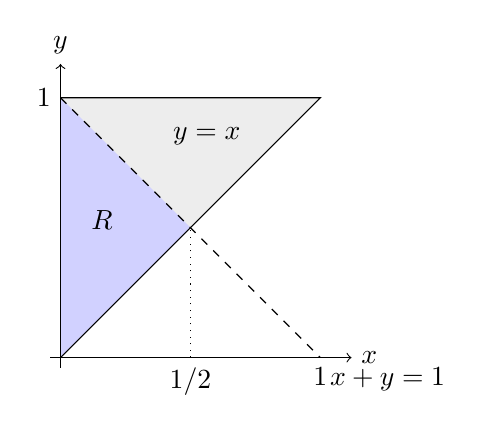
\begin{tikzpicture}[scale=3.3]
\fill[black!7] (0,0)--(0,1)--(1,1)--cycle;
\fill[blue!18] (0,0)--(0,1)--(.5,.5)--cycle;
\draw[->] (-.04,0)--(1.12,0) node[right]{$x$};
\draw[->] (0,-.04)--(0,1.13) node[above]{$y$};
\draw (0,0)--(1,1)--(0,1);
\draw[dashed] (0,1)--(1,0) node[below right]{$x+y=1$};
\draw[dotted] (.5,0)--(.5,.5);
\node[below] at (.5,0){$1/2$};
\node[below] at (1,0){$1$};
\node[left] at (0,1){$1$};
\node at (.16,.53){$R$};
\node[above left] at (.73,.78){$y=x$};
\end{tikzpicture}
\end{center}

\paragraph{A rectangle can still require a split.} On $0<x<1$, $0<y<2$, the event $X<Y$ can be written with one integral,
\[
 \int_0^1\int_x^2 f(x,y)\,\dd y\,\dd x,
\]
or with two integrals in the reverse order,
\[
 \int_0^1\int_0^y f(x,y)\,\dd x\,\dd y
 +\int_1^2\int_0^1 f(x,y)\,\dd x\,\dd y.
\]
For $0<y<1$, the line $x=y$ is the right boundary; for $1<y<2$, the rectangle's boundary $x=1$ takes over.

\paragraph{Checkpoint.} Let $f(x,y)=1/2$ on $0<x<1$, $0<y<2$. Write both orders and calculate $P(X+Y<1)$. \emph{Answer:} $\int_0^1\int_0^{1-x}\tfrac12\,\dd y\,\dd x=\int_0^1\int_0^{1-y}\tfrac12\,\dd x\,\dd y=1/4$.

\subsection{Translating word problems into events}

Name the random quantities and identify the logical operation before calculating. ``And'' is intersection; ``either'' usually includes the possibility that both occur unless explicitly excluded.

\begin{center}
\begin{tabular}{@{}p{0.48\linewidth}p{0.44\linewidth}@{}}
\toprule
Words & Mathematical event or quantity\\
\midrule
First component fails before the second & $X<Y$\\
Total cost is at most $b$ & $X+Y\leq b$\\
Costs differ by less than $d$ & $|X-Y|<d$\\
At least one fails by time $t$ & $\{X\leq t\}\cup\{Y\leq t\}$; equivalently $\min(X,Y)\leq t$\\
Both fail by time $t$ & $X\leq t,Y\leq t$; equivalently $\max(X,Y)\leq t$\\
Both still operate at time $t$ & $X>t,Y>t$\\
Reimbursement at least $a$ when spending is $x_0$ & $P(Y\geq a\mid X=x_0)$\\
Mean total payout after a policy change & $\E[aX+bY+c]$\\
Variability of that total & $\Var(aX+bY+c)$\\
\bottomrule
\end{tabular}
\end{center}

\paragraph{Series and parallel lifetimes.} A series device fails when \emph{either} component fails, so its lifetime is $T=\min(X,Y)$. A parallel device continues operating until \emph{both} have failed, so $T=\max(X,Y)$. Therefore,
\[
\begin{aligned}
P(\text{series failure by }t)
 &=1-P(X>t,Y>t)\\
 &=F_X(t)+F_Y(t)-F_{X,Y}(t,t),\\
P(\text{parallel failure by }t)&=F_{X,Y}(t,t).
\end{aligned}
\]
Only if independence is established may the first expression be replaced by $1-[1-F_X(t)][1-F_Y(t)]$, or the second by $F_X(t)F_Y(t)$.

\subsubsection*{Worked example: conditional reimbursement}
Suppose spending $X$ has density $f_X(x)=x/2$ for $0<x<2$ (hundreds of dollars), and reimbursement $Y$, given $X=x$, is uniform on $(0,x)$. Then
\[
 f_{Y\mid X}(y\mid x)=\frac1x\quad(0<y<x),\qquad
 f_{X,Y}(x,y)=\frac12\quad(0<y<x<2).
\]
``Reimbursed at least \$100 after spending \$150'' means
\[
 P(Y\geq1\mid X=1.5)=\int_1^{1.5}\frac{1}{1.5}\,\dd y=\frac13.
\]
The unit conversion must occur before selecting limits. The answer is conditional, so integrating the original joint density over a two-dimensional region would answer a different question.

\paragraph{Checkpoint.} A device fails if either component fails. Express ``the device lasts beyond two hours'' and ``the device fails within two hours'' in terms of $X,Y$. \emph{Answer:} The events are $\{X>2,Y>2\}$ and its complement $\{X\leq2\}\cup\{Y\leq2\}$.

\paragraph{Exam habits.} Write support and event; normalize; derive only the required marginal; divide by the given-variable marginal if conditioning; state the formula before inserting numbers; and check that a probability lies in $[0,1]$. On an independence question, write an actual equality proof or a specific probability-law counterexample.

\subsubsection*{Additional textbook practice, checked against Freund}
The following are references to the supplied eighth edition; the task descriptions are paraphrases. Use the problem statements in the textbook for their exact numerical data.
\begin{itemize}[leftmargin=*]
\item \textbf{Chapter 3, \S5, Exercises 42--43, p.~90:} read events and CDF values from a joint probability table. This is direct preparation for Homework~4, Problem~4.
\item \textbf{Chapter 3, \S5, Exercises 44--45, p.~90:} first normalize a polynomial joint PMF, then add selected cells for events involving both variables.
\item \textbf{Chapter 3, \S5, Exercise 50, p.~90:} integrate a polynomial density over a smaller triangle inside triangular support; useful for practicing changing limits.
\item \textbf{Chapter 3, \S5, Exercises 54--55 and 58, p.~91:} recover a density from a CDF and calculate a rectangle probability; derive the four-term rectangle identity.
\item \textbf{Chapter 3, \S7, Exercises 69--70, p.~100:} obtain marginals and conditionals from a joint table. Exercise~70 uses the table in Exercise~42.
\item \textbf{Chapter 3, \S7, Exercises 73--75, p.~100:} justify independence for discrete laws, then derive marginals and conditional densities on a rectangle. Exercises~74--75 use the same density as Homework~4, Problem~2.
\item \textbf{Chapter 3, \S7, Exercises 76--77, p.~100:} derive marginals on nonrectangular supports and decide independence. Exercise~76 matches the form of the optional STA~631 triangular homework problem after interchanging $x$ and $y$.
\item \textbf{Chapter 3, \S7, Exercise 79, p.~101:} recover a marginal CDF by letting the other CDF argument approach infinity.
\end{itemize}

